% XeLaTex
%\documentclass[review]{cvpr}
\documentclass[final]{cvpr}

\usepackage[UTF8]{ctex}

% \usepackage{cvpr}
\usepackage{times}
\usepackage{epsfig}
\usepackage{graphicx}
\usepackage{amsmath}
\usepackage{amssymb}
\usepackage{subfigure}
\usepackage{overpic}

\usepackage{enumitem}
\setenumerate[1]{itemsep=0pt,partopsep=0pt,parsep=\parskip,topsep=5pt}
\setitemize[1]{itemsep=0pt,partopsep=0pt,parsep=\parskip,topsep=5pt}
\setdescription{itemsep=0pt,partopsep=0pt,parsep=\parskip,topsep=5pt}

\usepackage[pagebackref=true,breaklinks=true,colorlinks,bookmarks=false]{hyperref}
\usepackage{listings} % 插入代码用到
% 用来设置附录中代码的样式
\lstset{
    breaklines=true,
	basicstyle          =   \footnotesize\sffamily,          % 基本代码风格
	flexiblecolumns,                % 别问为什么,加上这个
	showspaces          =   false,  % 是否显示空格,显示了有点乱,所以不现实了
	captionpos          =   t,      % 这段代码的名字所呈现的位置,t指的是top上面
	frame               =   lrtb,   % 显示边框
    showstringspaces=true,% 不显示字符串中的空格
}

\usepackage{hyperref}
\makeatletter
\def\UrlAlphabet{%
      \do\a\do\b\do\c\do\d\do\e\do\f\do\g\do\h\do\i\do\j%
      \do\k\do\l\do\m\do\n\do\o\do\p\do\q\do\r\do\s\do\t%
      \do\u\do\v\do\w\do\x\do\y\do\z\do\A\do\B\do\C\do\D%
      \do\E\do\F\do\G\do\H\do\I\do\J\do\K\do\L\do\M\do\N%
      \do\O\do\P\do\Q\do\R\do\S\do\T\do\U\do\V\do\W\do\X%
      \do\Y\do\Z}
\def\UrlDigits{\do\1\do\2\do\3\do\4\do\5\do\6\do\7\do\8\do\9\do\0}
\g@addto@macro{\UrlBreaks}{\UrlOrds}
\g@addto@macro{\UrlBreaks}{\UrlAlphabet}
\g@addto@macro{\UrlBreaks}{\UrlDigits}
\makeatother

\newcommand{\cmm}[1]{\textcolor[rgb]{0,0.6,0}{CMM: #1}}
\newcommand{\todo}[1]{{\textcolor{red}{\bf [#1]}}}
\newcommand{\alert}[1]{\textcolor[rgb]{.6,0,0}{#1}}
\newcommand{\mypara}[1]{\paragraph{#1.}}

\graphicspath{{figures/}}

\begin{document}
% \begin{CJK*}{GBK}{song}

\renewcommand{\figref}[1]{图\ref{#1}}
\renewcommand{\tabref}[1]{表\ref{#1}}
\renewcommand{\equref}[1]{式\ref{#1}}
\renewcommand{\secref}[1]{第\ref{#1}节}
\def\abstract{\centerline{\large\bf 摘要} \vspace*{12pt} \it}

%%%%%%%%% TITLE

\title{操作系统课程报告:虚拟机的安装与使用}

\author{张昊  \quad 1927405160 \\ 苏州大学计算机科学与技术学院19级图灵班
}

\maketitle
% \thispagestyle{empty}

%%%%%%%%% ABSTRACT
\begin{abstract}
虚拟机指通过软件模拟的具有完整硬件系统功能的、运行在一个完全隔离环境中的完整计算机系统。本文基于工作站虚拟机软件 Oracle VM Virtual Box ,介绍了虚拟机的安装与使用,并根据实际操作的过程中遇到的问题进行了总结和整理。
\end{abstract}

%%%%%%%%% BODY TEXT %%%%%%%%%%%%%%%%%%%%%%%%%%%%%%%%%%%%%%%%
\section{引言}\label{sec:Introduction}

虚拟机(Virtual Machine)指通过软件模拟的具有完整硬件系统功能的、运行在一个完全隔离环境中的完整计算机系统,可以分为高级语言虚拟机、工作站虚拟机和服务器虚拟机。
工作站虚拟机是较为常用的一种虚拟机,它是一种安装在操作系统上的虚拟机,在工作站虚拟机中可以安装客户操作系统(Guest OS),使得用户可以同时在一个计算机上使用多个操作系统。
通过工作站虚拟机软件,用户可以在一台物理计算机上模拟出多台虚拟的计算机,这些虚拟机完全就像真正的计算机那样进行工作,例如安装操作系统、安装应用程序、访问网络资源等等。

本文主要讨论了以下三个内容:

\begin{itemize}
\item 在宿主操作系统(Host OS)中安装工作站虚拟机软件;
\item 使用工作站虚拟机软件安装主流操作系统;
\item 使用虚拟机的一些常见问题与解决办法。
\end{itemize}

本文基于Oracle VM Virtual Box\cite{Web/VirtualBox}这一开源虚拟机软件,
宿主操作系统选用Windows 8.1企业版(硬件环境为 Intel(R) Core(TM) i5-6500 CPU,16.0 GB 内存),分别安装了Ubuntu 20.04以及macOS 10.15 Catalina两个虚拟机。
简要地总结一下后续章节的内容,
第\ref{sec:RelatedWorks}章介绍了目前网络上搜集到的有关工作站虚拟机的一些资料,
第\ref{sec:installVBox}章介绍了Oracle VM Virtual Box\cite{Web/VirtualBox}的在Windows系统下的安装方法,
第\ref{sec:ubuntu}章和第\ref{sec:mac}章分别介绍了Ubuntu 20.04以及macOS 10.15 Catalina两个虚拟机的安装流程,以及使用过程中遇到的问题与解决办法,并在第\ref{sec:Conclusion}章进行了总结。

%%%%%%%%%%%%%%%%%%%%%%%%%%%%%%%%%%%%%%%%%%%%%%%%%%%%%%%%%%%%%%%%%%%%%%%%%%%%%%%
\section{相关资料}
\label{sec:RelatedWorks}

本文主要关注工作站虚拟机的相关资料。在网络上可以搜集到的资料中,大多数都是介绍工作站虚拟机的安装与使用。

面向不同的宿主操作系统,主流的工作站虚拟机软件有
VMware Workstation、Virtual Box、Parallels Desktop等。

\begin{itemize}
\item VMware Workstation是一款收费的工作站虚拟机软件,可以运行在 Windows 或 Linux PC 上(VMware 在 macOS 平台上提供类似的产品 VMware  Fusion),以支持在一台电脑上同时运行多个虚拟机,用于代码开发、解决方案构建、应用测试、产品演示等\cite{Web/VMwareWorkstation}。
\item Oracle VM Virtual Box 是由 Oracle 开发的一款 x86 和 AMD64/Intel64 虚拟化产品,适用于企业和家庭使用。VirtualBox 是一款基于 GNU 通用公共许可证 (GPL) 第 2 版的条款的开源软件,免费为企业和个人用户提供解决方案\cite{Web/VirtualBox},可以运行在 Windows、Linux、Macintosh 和 Solaris 平台上。
\item Parallels Desktop\cite{Web/ParallelsDesktop} 是由 Parallel 推出的一款为使用英特尔处理器以及M1处理器的苹果电脑提供硬件虚拟化的软件。用户可以通过 Parallels Desktop for Mac 在苹果电脑上安装 Windows、Linux 发行版、FreeBSD、MS-DOS、EComStation、OS/2、Solaris 等系统。同样,Parallels Desktop也是一款收费的工作站虚拟机软件。
\end{itemize}

安装在操作系统上的操作系统称为客户操作系统(Guest OS)。
像Virtual Box这一类虚拟机,使用到了虚拟化(Virtualization)技术,这通常需要CPU支持(如Intel VT-x、AMD-V)。
客户操作系统的CPU架构是与宿主操作系统相同的,即如果宿主操作系统运行在x86的处理器上,虚拟机几乎可以支持所有运行在x86处理器上的客户操作系统。
还有一些虚拟机使用到了仿真(Emulation),如QEMU\cite{Web/QEMU},可以在任何支持的体系结构上运行任意的操作系统\footnote{严格来说,QEMU有三种运行模式:Full-system emulation模式可在任何支持的硬件架构上运行任何操作系统;User-mode emulation模式可以运行不同目标架构的 Linux/BSD 程序;Virtualization模式可以接近本机性能运行 KVM 和 Xen 虚拟机\cite{Web/QEMU}。其中前两种模式使用了仿真,后一种模式使用的是虚拟化技术;Full-system emulation模式和Virtualization模式更接近工作站虚拟机的概念。}。

%%%%%%%%%%%%%%%%%%%%%%%%%%%%%%%%%%%%%%%%%%%%%%%%%%%%%%%%%%
\section{Virtual Box 的安装}\label{sec:installVBox}

首先,访问Virtual Box官方网站\footnote{请访问Virtual Box官方网站:\url{https://www.virtualbox.org/wiki/Downloads/}。 }
下载最新版本的安装包,根据自己的系统下载对应的版本。如\figref{fig:download},这里下载Windows主机系统的6.1.26版本。
\begin{figure}
  	\begin{overpic}[width=\columnwidth]{install-download.png}\end{overpic}
    \caption{Virtual Box官网下载。}\label{fig:download}
\end{figure}
双击打开或者管理员身份运行VirtualBox-***-win.exe,打开安装向导,点击“下一步 >”,进入下一步。\figref{fig:install1}所示界面可以选择要安装的功能组件,按顺序分别是:
\begin{itemize}
    \item 主程序(必选);
    \item Virtual Box USB驱动支持(用以支持外部USB设备连接到虚拟机);
    \item 虚拟机的网络支持(桥接与主机模式的网络);
    \item Virtual Box的Python 2.X的支持。
\end{itemize}
可以根据需求调整各组件的安装情况与安装位置,这里使用默认配置。安装路径默认在系统盘,点击“ 浏览 ”选择其他的安装路径,然后点击“下一步 >”,进入下一步。
\begin{figure}
  	\begin{overpic}[width=\columnwidth]{install-1.png}\end{overpic}
    \caption{Virtual Box安装向导组件选择。}\label{fig:install1}
\end{figure}

此后是快捷方式的选项,可根据个人习惯选择。在安装虚拟网络组件时会弹出警告界面,提示安装网络组件会重置当前网络(如\ref{fig:install-warnning}),选择“是”,并完成后续安装步骤即可,这里不在赘述。
\begin{figure}
  	\begin{overpic}[width=\columnwidth]{install-warnning.png}\end{overpic}
    \caption{虚拟网络组件安装警告界面。}\label{fig:install-warnning}
\end{figure}

\mypara{说明}  在安装过程中会弹出如\ref{fig:install-notice}所示的设备安装界面,都选择“安装”,如果这里选择不安装会对之后的USB设备、网络的使用有影响。
\begin{figure}
  	\begin{overpic}[width=\columnwidth]{install-notice.png}\end{overpic}
    \caption{设备安装界面(图片来源于网络)\cite{Web/installVB}。}\label{fig:install-notice}
\end{figure}

%%%%%%%%%%%%%%%%%%%%%%%%%%%%%%%%%%%%%%%%%%%%%%%%%%%%%%%%%%
\section{Ubuntu 虚拟机的安装}\label{sec:ubuntu}

Ubuntu 虚拟机的创建与安装较为简单,我们需准备好系统镜像,并预留有约50 GB的磁盘空间即可。


%%%%%%%%%%%%%%%%%%%%%%%%%%%%%%%%%%%%%%%%%%%%%%%

\subsection{\textbf{操作系统镜像下载}}\label{sec:download-ubuntu-image}

我们可以访问Ubuntu官方网站下载Ubuntu系统镜像\footnote{Ubuntu Desktop :\url{https://ubuntu.com/download/desktop/}。},这里我们选择下载Ubuntu Desktop 20.04.03 LTS,如\figref{fig:ubuntu-download}所示。

\begin{figure}
  	\begin{overpic}[width=\columnwidth]{ubuntu-download.png}\end{overpic}
    \caption{Ubuntu Desktop系统镜像下载。}\label{fig:ubuntu-download}
\end{figure}

%%%%%%%%%%%%%%%%%%%%%%%%%%%%%%%%%%%%%%%%%%%%%%


\subsection{\textbf{虚拟机安装与配置}}


\begin{figure*}[t]
  \centering
  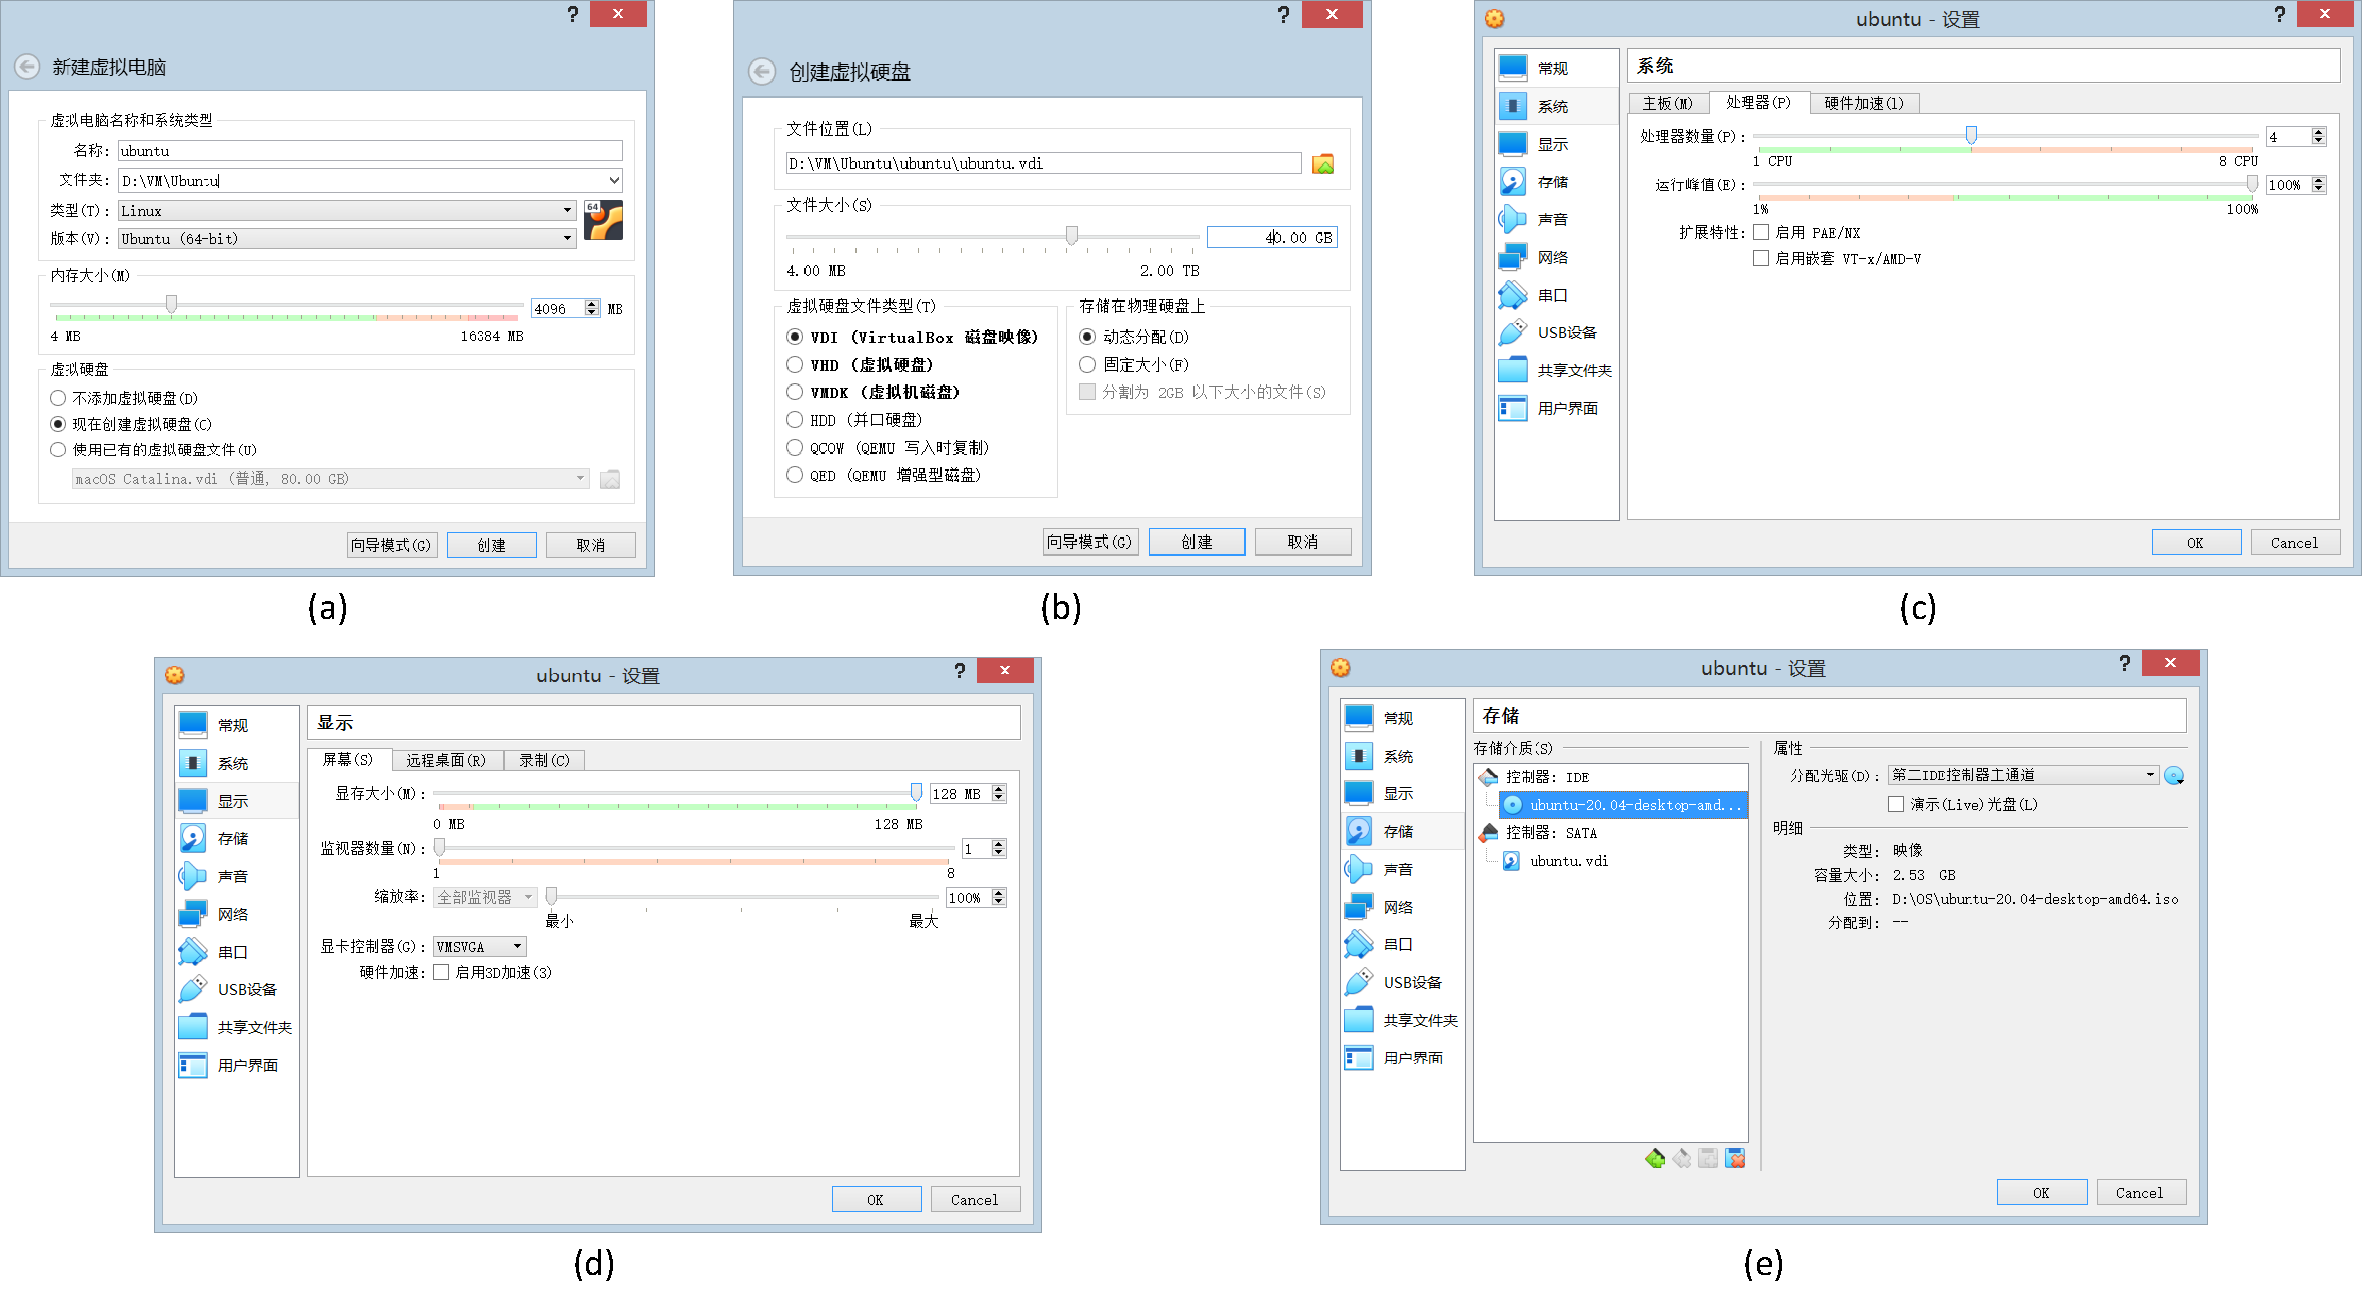
\includegraphics[width=\textwidth]{ubuntu-i1.pdf}
  \caption{虚拟机的创建与配置。\textit{新建一个名为“ubuntu”的虚拟机,设置其类型为“Linux”-“Ubuntu (64-bit)”,并选定虚拟机保存的位置。
  为虚拟机分配4096 MB的内存空间,40 GB的虚拟磁盘空间,并设置虚拟磁盘的存储为动态分配。
  保存虚拟机后,点击“设置”,对虚拟机的硬件进行进一步的配置:设置处理器数量为4,运行峰值100\%,显存大小为128 MB。
  并将\ref{sec:download-ubuntu-image}节下载的镜像添加到存储介质中作为虚拟光盘。}}\label{fig:ubuntu-config}
\end{figure*}

\begin{figure*}[t]
  \centering
  \begin{overpic}[width=\textwidth]{install-ubuntu1-2.png}\end{overpic}
  \caption{开始安装Ubuntu操作系统。\textit{系统镜像加载后,选择语言为“中文(简体)”,点击“安装 Ubuntu”,并选定键盘布局。为减少安装操作系统时的耗时,在“您希望安装哪些应用”中选择“最小安装”,“其他选项”中取消勾选“安装Ubuntu时下载更新”。安装类型可选择全盘安装和自定义两种。}}\label{fig:install-ubuntu1}
\end{figure*}

\begin{figure*}[t]
  \centering
  \begin{overpic}[width=\textwidth]{install-ubuntu2-1.png}\end{overpic}
  \caption{开始安装Ubuntu操作系统。\textit{确认安装类型后,会提示硬盘分区表修改,点击“继续”,创建Linux用户后,安装程序就开始了操作系统的安装。当右下角的“skip”可点击后,可以点击“skip”跳过一些软件包的安装,以减少安装操作系统时的耗时。当操作系统安装完成后,会提示重启。}}\label{fig:install-ubuntu2}
\end{figure*}

\mypara{第一步}  按\figref{fig:ubuntu-config}所示流程创建并配置虚拟机。

\begin{itemize}
    \item 打开Virtual Box ,点击"新建"按钮,在专家模式下选择虚拟机类型为Linux,内存配置大于1 GB,并选择虚拟机保存的位置。
    \item 创建磁盘容量的时候一定要大于20 GB(这里设置40GB的磁盘空间),否则后续安装系统的过程可能会出现问题。
    \item 创建完成后,选中创建好的虚拟机,点击“设置”,对虚拟机的硬件(CPU核心数、运行峰值、显存大小等)进行进一步的配置。
    \item 最后在“存储”标签页中将\ref{sec:download-ubuntu-image}节下载的镜像添加到存储介质中作为虚拟光盘。
\end{itemize}

创建好虚拟机后,我们可以看到如\figref{fig:ubuntu-vbox}所示的虚拟机配置。点击“启动”,打开虚拟机电源并安装操作系统。

\begin{figure}
  	\begin{overpic}[width=\columnwidth]{ubuntu6.PNG}\end{overpic}
    \caption{Virtual Box中创建好的Ubuntu虚拟机。点击“启动”打开虚拟机电源。}\label{fig:ubuntu-vbox}
\end{figure}

\mypara{第二步}  按\figref{fig:install-ubuntu1}和\figref{fig:install-ubuntu2}所示流程安装虚拟机的操作系统。

系统镜像加载后,选择语言并点击“安装 Ubuntu”,选定键盘布局。
为减少安装操作系统时的耗时,在“您希望安装哪些应用”中选择“最小安装”,“其他选项”中取消勾选“安装Ubuntu时下载更新”。
这样做是由于Ubuntu的默认的apt软件源在国内访问速度不佳,会造成安装操作系统过程中漫长的等待。
同时,也可以使得安装的Ubuntu尽可能小,其他可选功能后续可以按需安装。

安装类型可选择全盘安装和自定义两种。全盘安装会格式化整个磁盘,并按照默认的配置进行分区。如果对文件系统的挂载点\footnote{简单来说,挂载点实际上就是Linux中的磁盘文件系统的入口目录,类似于Windows中的用来访问不同分区的C:、D:、E:等盘符。}或者磁盘文件系统类型有要求,可以在自定义(“其他选项”)中自行改动,如\figref{fig:ubuntu-disk}所示。

\begin{figure}
  	\begin{overpic}[width=\columnwidth]{ubuntu-disk-1.png}\end{overpic}
    \caption{手动调整分区表以及Linux的挂载点。}\label{fig:ubuntu-disk}
\end{figure}

确认安装类型后,会提示硬盘分区表修改,点击“继续”,创建Linux用户后,安装程序就开始了操作系统的安装。

同样是为了减少安装操作系统时的耗时,当右下角的“skip”可点击后,可以点击“skip”跳过一些软件包的安装。当操作系统安装完成后,会提示重启。如果是使用Live系统
\footnote{Live系统,即Ubuntu Live CD,是刻录在光盘上运行的Linux,
是一套已经装好的系统,其中也有在硬盘上安装系统的选项。
可以使Ubuntu系统从光盘启动,用户可以方便的先对系统进行一次体验,再进行硬盘安装。 }
安装的会询问是否继续留在Live系统。

至此,Ubuntu虚拟机的操作系统就已经安装完成了,如\figref{fig:ubuntu-finfish}所示。

\begin{figure}
  	\begin{overpic}[width=\columnwidth]{ubuntu-finfish-1.png}\end{overpic}
    \caption{Ubuntu操作系统安装完成。}\label{fig:ubuntu-finfish}
\end{figure}

\subsection{\textbf{问题与解决}}

\mypara{问题}  有时虚拟机的分辨率过低,\figref{fig:install-ubuntu1}所示的下方的按钮被遮挡而无法显示。

此时可以进入到Live系统中调整屏幕的分辨率,并安装操作系统。如\figref{fig:ubuntu-live}所示,可以通过在系统安装界面关闭安装程序,或者在系统镜像加载后,选择语言并点击“试用 Ubuntu”,来进入Live系统。在Live系统中点击右上角-“设置”-“显示器”,调整屏幕分辨率。实测分辨率大于1024×768时不会出现按钮遮挡的问题。

\begin{figure}
  	\begin{overpic}[width=\columnwidth]{ubuntu-live-1.png}\end{overpic}
    \caption{在Ubuntu Live 系统中调整屏幕分辨率。}\label{fig:ubuntu-live}
\end{figure}


%%%%%%%%%%%%%%%%%%%%%%%%%%%%%%%%%%%%%%%%%%%%%%%%%%%%%%%%%%
\section{macOS 10.15 Catalina 虚拟机的安装}\label{sec:mac}

相较于 Ubuntu 虚拟机的安装,macOS 虚拟机的安装稍显复杂,
原因在于 macOS 并不会对外公开 iso 格式的系统镜像的下载,
并且macOS是专为Mac电脑设计的,在虚拟机中可能存在一些兼容性问题,需要一一调整。
我们需准备好系统镜像,并预留有约100 GB的磁盘空间即可。

%%%%%%%%%%%%%%%%%%%%%%%%%%%%%%%%%%%%%%%%%%%%%%%%%%%%%%%%%%
\subsection{\textbf{操作系统镜像下载与制作}}\label{sec:install-image}

在Virtual Box中安装任何系统,都需要有相应的iso镜像文件,所以首先要获取macOS 10.15 Catalina的iso镜像文件。有两种解决方案:如果有现成可用的运行着macOS 10.15 Catalina系统的电脑(包括MacBook、iMac、虚拟机等),可以使用如下所述的方法来自行打包镜像;否则,需要到网络上搜索并下载他人打包好的镜像\footnote{这里提供一个百度网盘的资源\cite{Web/installCatalina}:链接 \url{https://pan.baidu.com/s/1oCIbO6tMwcwmFxVZc_SfZA} ,提取码 cz6j。}。
接下来将介绍第一种解决方案,在一台MacBook Pro 上制作系统镜像的流程。

\mypara{第一步}  从Mac App Store下载最新的Catalina系统。
在App Store中搜索Catalina系统,如\figref{fig:catalina-app-store},点击“获取”。
\begin{figure}
  	\begin{overpic}[width=\columnwidth]{app-store.png}\end{overpic}
    \caption{在App Store中搜索Catalina系统,并获取系统镜像。}\label{fig:catalina-app-store}
\end{figure}
如果App Store中搜索不到Catalina系统,可以使用Safari浏览器访问链接
{ \small { \url{https://apps.apple.com/cn/app/macos-catalina/id1466841314?mt=12&irgwc=1&aosid=p239&cid=aos-cn-aff-ir&irchannel=13654&irpid=1244234&clickid=3GtS30WxDxyJRTI0EBxnPXevUkn2VC2MZwz6Uc0&ircid=7639} } }
,即可进入下载界面。

\mypara{第二步}  制作iso镜像。

参考资料\cite{Web/installCatalina}中的做法。\footnote{
本文代码块中所有出现在字符串外的反斜杠$\backslash$均为续行符。
}

\begin{itemize}
    \item 在Mac App Store中下载的应用一般会保存在根目录下的资源库(Applications 目录)中。
          打开终端,定位目录到资源库。
\begin{lstlisting}
% cd /Applications
\end{lstlisting}
    \item 创建一个空白的虚拟磁盘镜像,命名为temp,保存在当前目录下,
    设置初始大小不小于下载的 Install macOS Catalina.app文件的大小。
\begin{lstlisting}
% hdiutil create -o ./temp -size 8500m \
    -layout SPUD -fs HFS+J
\end{lstlisting}
    \item 将创建的虚拟磁盘镜像挂载到系统中,挂载点设置为 \lstinline{/Volumes/install_build} 。
\begin{lstlisting}
% hdiutil attach ./temp.dmg -noverify \
    -mountpoint /Volumes/install_build
\end{lstlisting}
    \item 使用 macOS createinstallmedia 工具为我们之前创建的虚拟磁盘镜像创建一个安装镜像。
    这一步需要root权限,需使用sudo命令(需要输入当前用户口令)。
\begin{lstlisting}
% sudo Install\ macOS\ Catalina.app/Contents\
    /Resources/createinstallmedia \
    --volume /Volumes/install_build 
\end{lstlisting}
    这一步会使得虚拟磁盘镜像的名称变为 Install macOS Catalina。
    \item 卸载该虚拟磁盘镜像:
\begin{lstlisting}
% hdiutil detach /Volumes/Install\ macOS\ Catalina/
\end{lstlisting}
    \item 将该虚拟磁盘镜像temp.dmg转换为cdr文件,会生成一个Catalina.cdr文件。
\begin{lstlisting}
% hdiutil convert temp.dmg -format UDTO -o Catalina
\end{lstlisting}
    \item 移动并且重命名。
\begin{lstlisting}
% mv Catalina.cdr Catalina.iso
\end{lstlisting}
\end{itemize}

至此,我们就获得了一个macOS 10.15 Catalina的系统镜像。
可以将其从这台Mac电脑中拷贝出来,转移到我们安装虚拟机的电脑中。

%%%%%%%%%%%%%%%%%%%%%%%%%%%%%%%%%%%%%%%%%%%%%%%%%%%%%%%%%%

\subsection{\textbf{虚拟机安装与配置}}

\begin{figure*}[t]
  \centering
  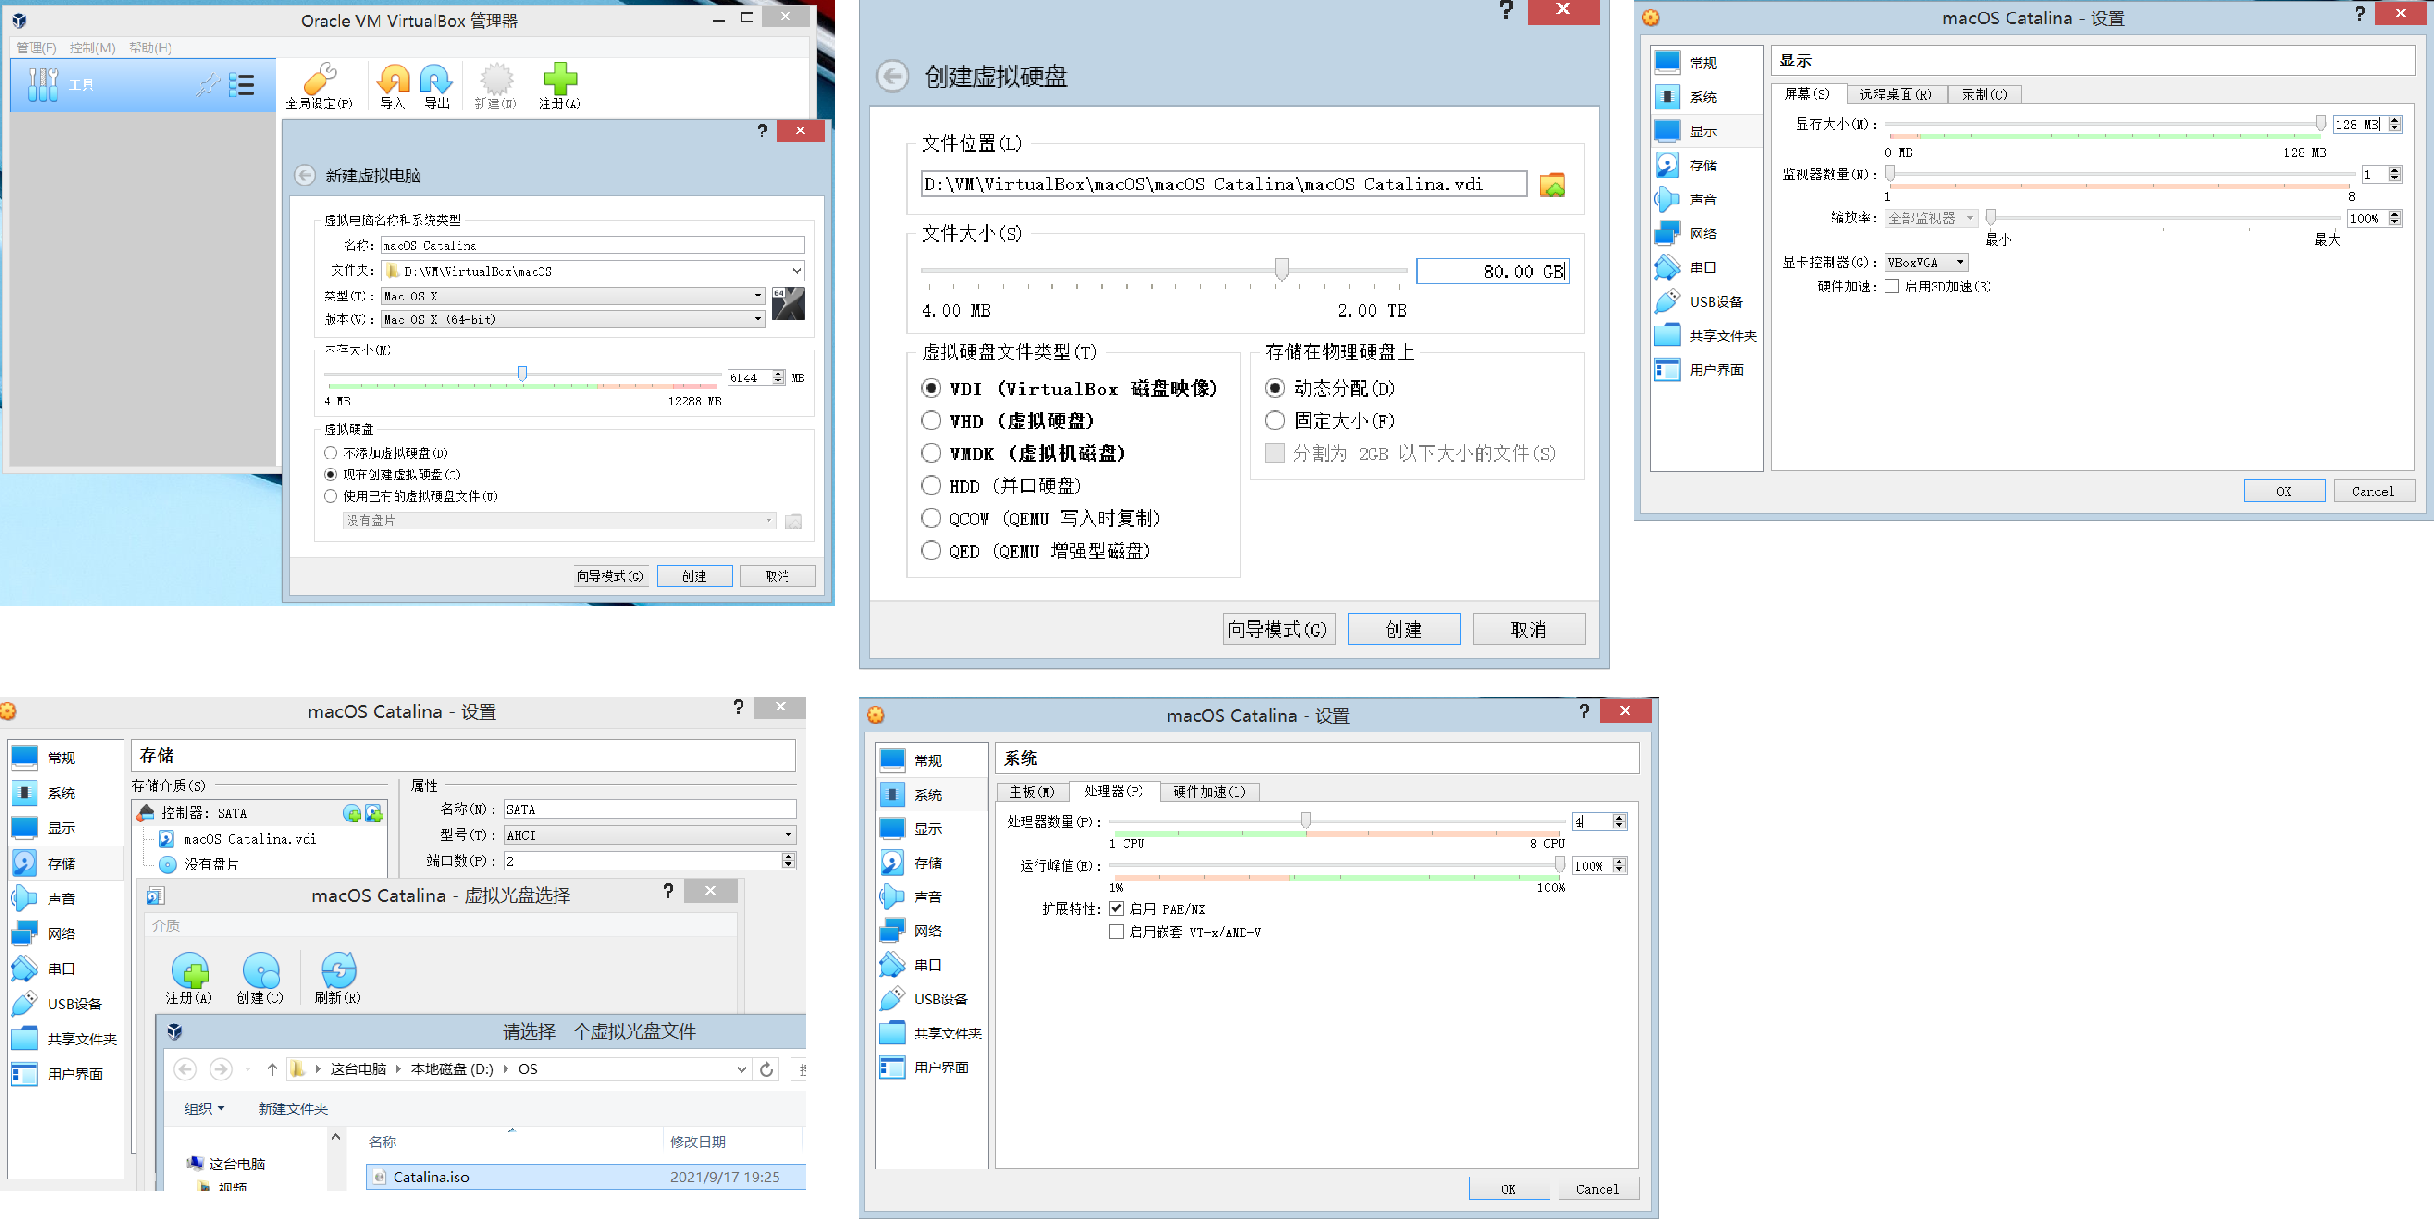
\includegraphics[width=\textwidth]{config.pdf}
  \caption{虚拟机的创建与配置。\textit{新建一个名为“macOS Catalina”的虚拟机,设置其类型为“Mac OS X”-“Mac OS X (64-bit)”,并选定虚拟机保存的位置。
  为虚拟机分配6144 MB的内存空间,80 GB的虚拟磁盘空间,并设置虚拟磁盘的存储为动态分配。
  保存虚拟机后,点击“设置”,对虚拟机的硬件进行进一步的配置:设置显存大小为128 MB,处理器数量为4,运行峰值100\%。
  并将\ref{sec:install-image}节制作的镜像添加到存储介质中作为虚拟光盘。 }}\label{fig:config}
\end{figure*}

\mypara{第一步}  按\figref{fig:config}所示流程创建并配置虚拟机。

\begin{itemize}
    \item 打开Virtual Box ,点击"新建"按钮,在专家模式下选择虚拟机类型为Mac OS X,内存配置大于4 GB,并选择虚拟机保存的位置。
    \item 创建磁盘容量的时候一定要大于25 GB(这里设置80GB的磁盘空间),否则后续安装系统的过程可能会出现问题。
    \item 创建完成后,选中创建好的虚拟机,点击“设置”,对虚拟机的硬件(CPU核心数、运行峰值、显存大小等)进行进一步的配置。
    \item 最后在“存储”标签页中将\ref{sec:install-image}节制作的镜像添加到存储介质中作为虚拟光盘。
\end{itemize}

\begin{figure*}[t]
  \centering
  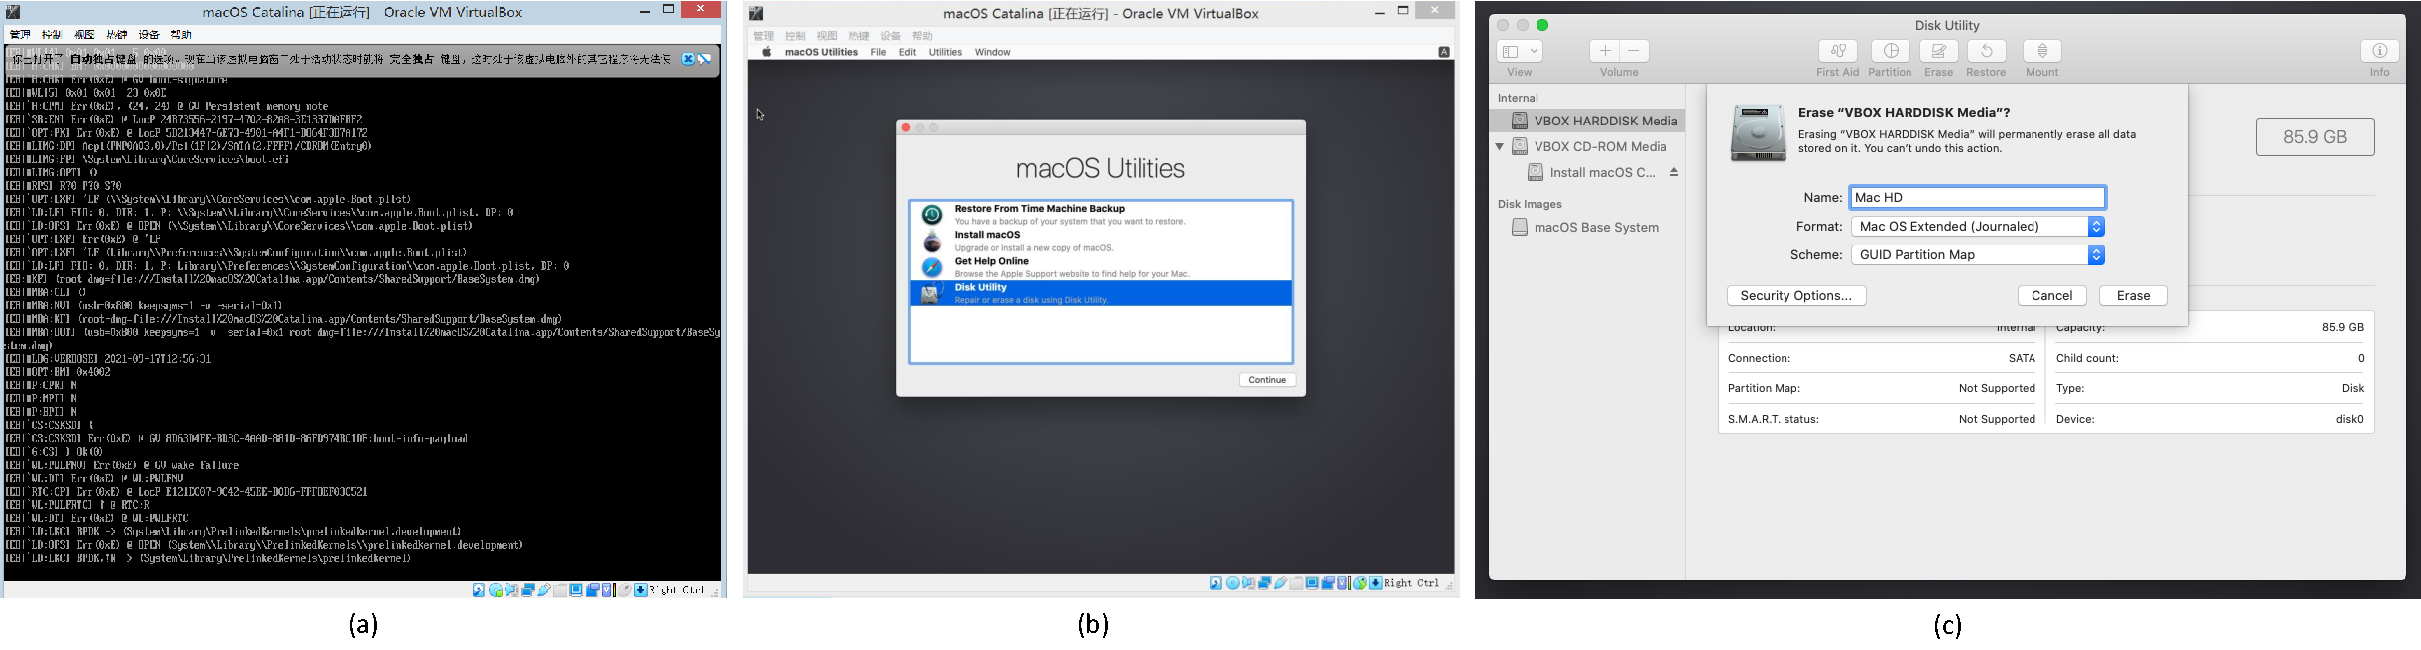
\includegraphics[width=\textwidth]{install1.pdf}
  \caption{配置虚拟机的硬盘。\textit{打开创建的虚拟机,首先会出现图(a)所示界面,大概持续3-4分钟左右(如果一直循环则安装出现了问题)。若启动正常则会进入语言选择界面,这里选择默认的英语。
  进入到图(b)所示的“macOS Utilities”界面,首先点击“Disk Utility”,进入图(c)所示的界面。选择以“VBOX”为前缀的磁盘,点击上方的“Erase”格式化该硬盘,
  在弹出的对话框中输入卷标(Name),选择格式为“Mac OS Extended (Journaled)”,模式(Scheme)保持默认的“GUID”,执行格式化。}}\label{fig:install1}
\end{figure*}

\begin{figure*}[t]
  \centering
  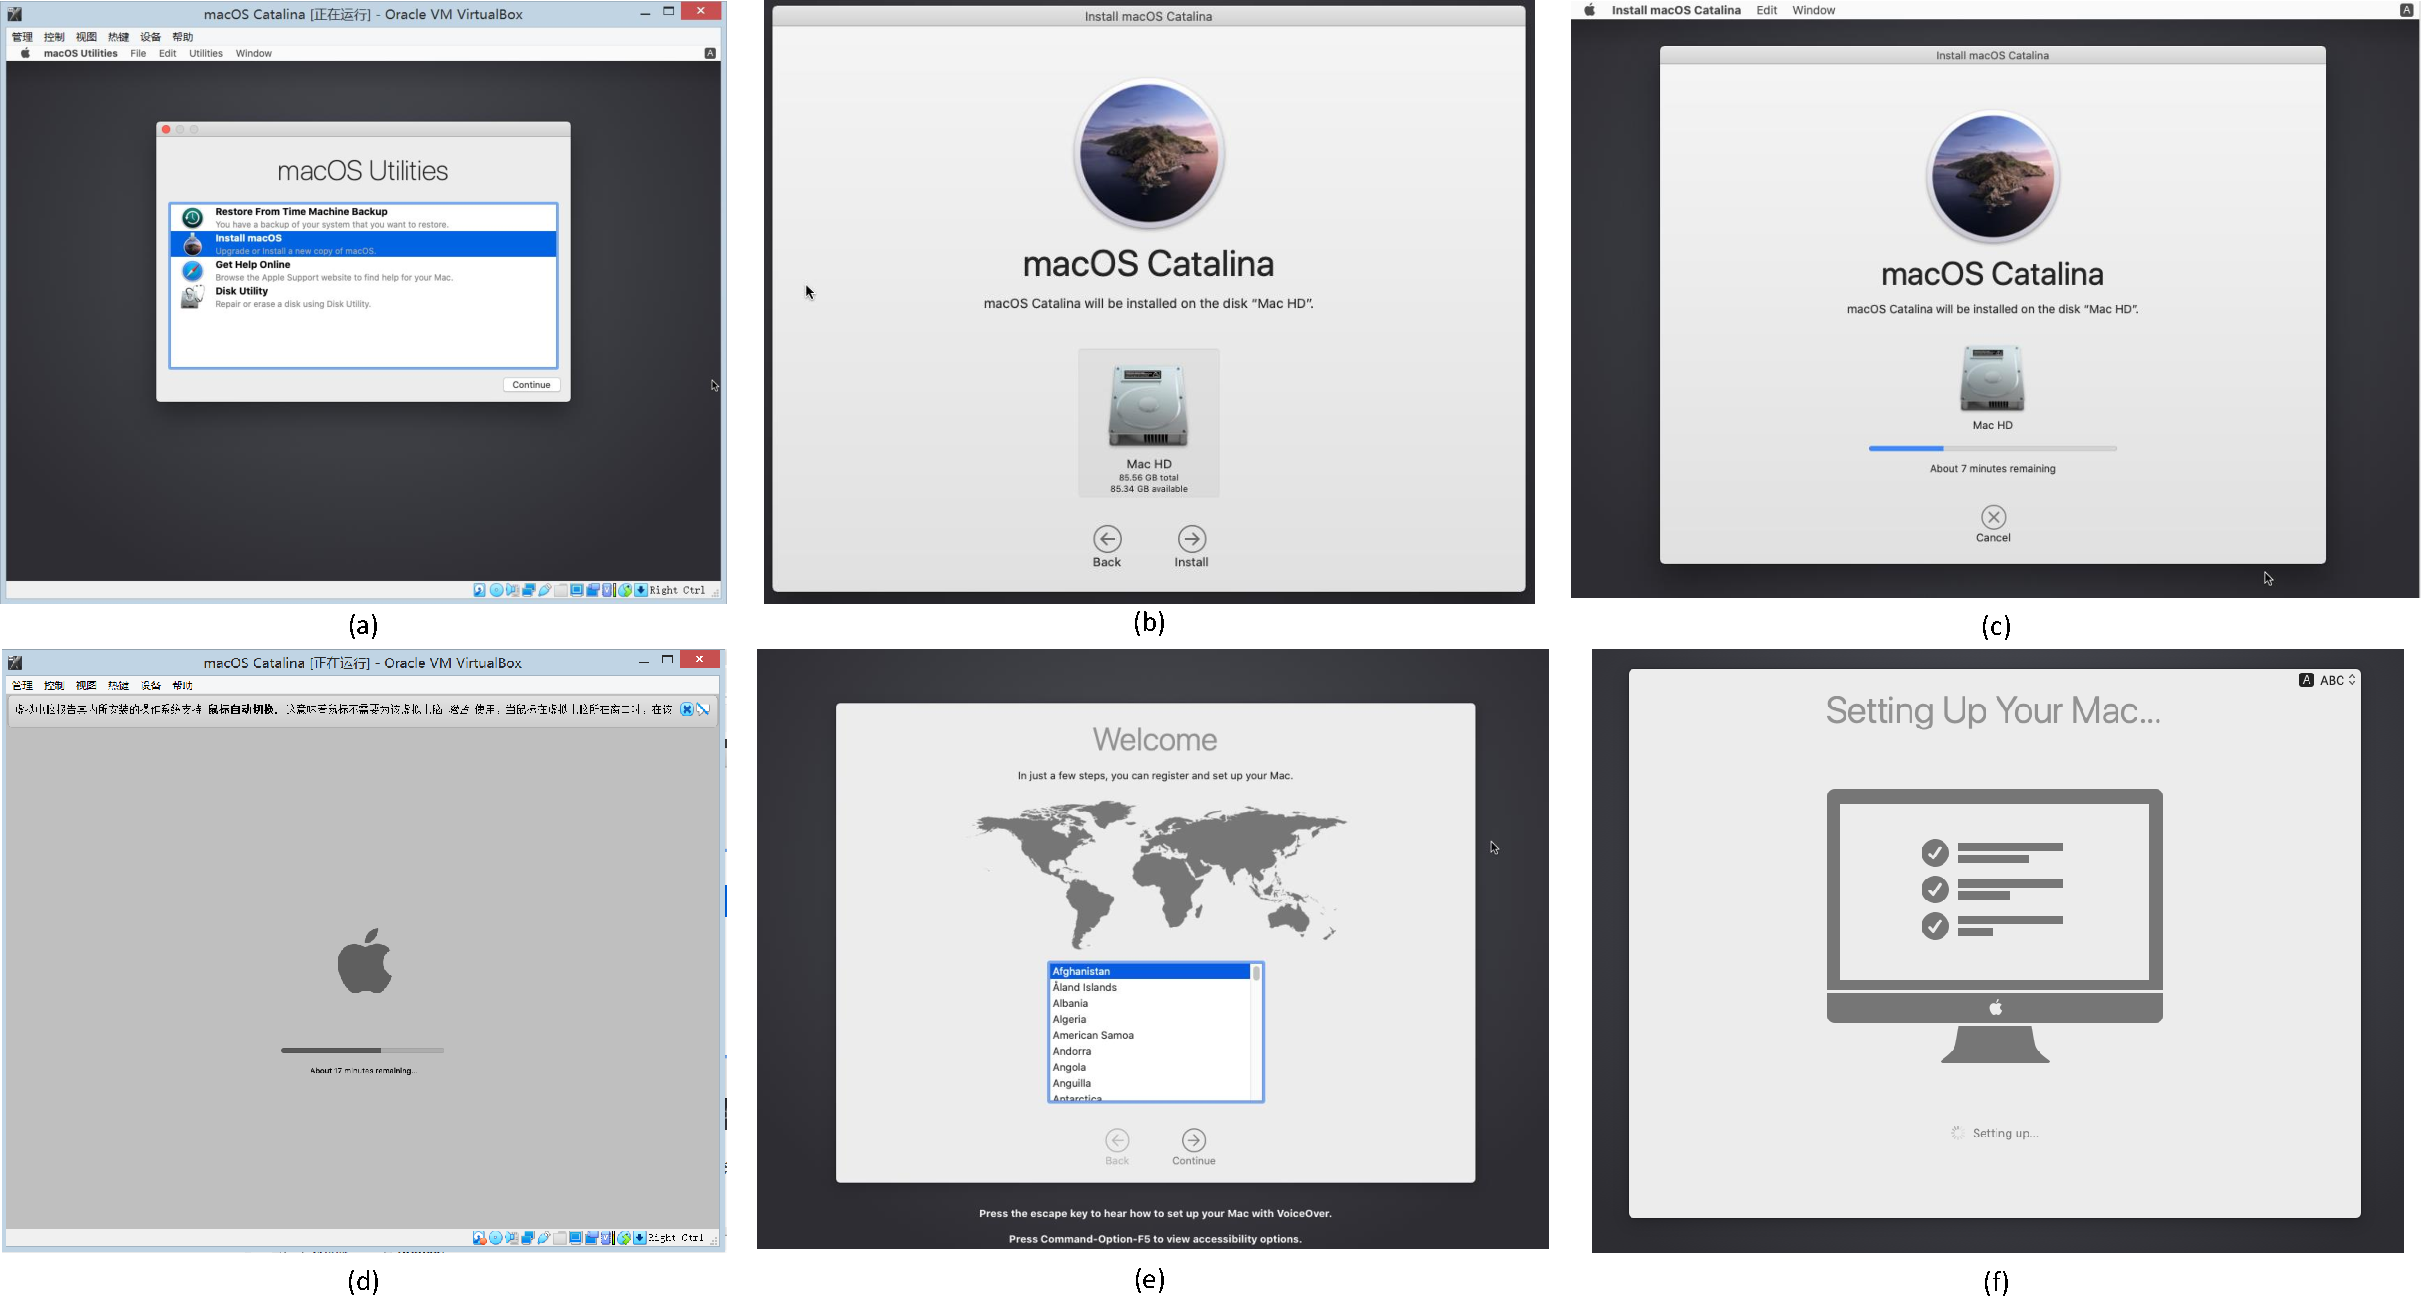
\includegraphics[width=\textwidth]{install2.pdf}
  \caption{安装虚拟机操作系统。\textit{在图(a)所示的“macOS Utilities”界面中点击“Install macOS”安装操作系统。
  如图(b)所示,选择之前格式化好的硬盘,安装程序将进行自动的安装,期间会重启一次,在图(c)、图(d)所示界面耐心等候。
  以上步骤都成功的完成后,macOS就安装好了,但是在开始使用前须进行一些系统初始化的操作,如图(e)、图(f)所示。}}\label{fig:install2}
\end{figure*}


\mypara{第二步} 为Virtual Box 添加额外配置项。

为使Virtual Box的虚拟机可以顺利安装macOS操作系统,需要在其安装目录下执行如下操作\cite{Web/installCatalina}:
首先关掉虚拟机以及 Virtual Box,以管理员权限运行命令提示符(或Power Shell)。将运行目录定位到Virtual Box的安装目录
\footnote{默认安装目录为 C:$\backslash$Program Files$\backslash$Oracle$\backslash$VirtualBox$\backslash$ 。 }。
\begin{lstlisting}
> cd "C:\Program Files\Oracle\VirtualBox\"
\end{lstlisting}
在此目录下执行如下操作:
\begin{lstlisting}
> VBoxManage modifyvm "macOS Catalina" --cpuidset \
    00000001 000106e5 00100800 0098e3fd bfebfbff
> VBoxManage setextradata "macOS Catalina" "VBoxInternal/\
    Devices/efi/0/Config/DmiSystemProduct" "iMac11,3"
> VBoxManage setextradata "macOS Catalina" "VBoxInternal/\
    Devices/efi/0/Config/DmiSystemVersion" "1.0"
> VBoxManage setextradata "macOS Catalina" "VBoxInternal/\
    Devices/efi/0/Config/DmiBoardProduct" "Iloveapple"
> VBoxManage setextradata "macOS Catalina" "VBoxInternal/\
    Devices/smc/0/Config/DeviceKey" \
    "ourhardworkbythesewordsguardedpleasedontsteal(c)\
    AppleComputerInc"
> VBoxManage setextradata "macOS Catalina" "VBoxInternal/\
    Devices/smc/0/Config/GetKeyFromRealSMC" 1
\end{lstlisting}
其中"macOS Catalina"为创建macOS虚拟机时设置的名称。
如\figref{fig:macOS6}所示。

\begin{figure}
  	\begin{overpic}[width=\columnwidth]{macOS6.PNG}\end{overpic}
    \caption{为Virtual Box 添加额外配置项。}\label{fig:macOS6}
\end{figure}

\mypara{第三步} 将macOS Catalina安装到虚拟机。

\begin{itemize}
    \item 首先按照\figref{fig:install1}格式化虚拟机的硬盘。启动Virtual Box,打开创建的虚拟机。
待启动成功后,在“macOS Utility”中选择“Disk Utility”,将以“VBOX”为前缀的磁盘格式化为“Mac OS Extended (Journaled)”格式。

    \item 成功格式化后,按照\figref{fig:install2}安装操作系统。在“macOS Utility”中选择“Install macOS”。
将系统安装到格式化好的硬盘(卷标为格式化时填写的),期间会有一次重启。待系统安装成功后将进行初次使用系统的一些初始化的操作。

\end{itemize}

至此,macOS Catalina就已经安装到了虚拟机中,可以看到虚拟机已经显示系统桌面(如\figref{fig:macOS17})。

\begin{figure}
  	\begin{overpic}[width=\columnwidth]{macOS17.PNG}\end{overpic}
    \caption{系统桌面。\textit{此时系统提示需要进行键盘布局的检测。}}\label{fig:macOS17}
\end{figure}


%%%%%%%%%%%%%%%%%%%%%%%%%%%%%%%%%%%%%%%%%%%%%%%%%%%%%%%%%%%%%%%%%%%%%%
\subsection{\textbf{问题与解决}}
\mypara{问题1}  虚拟机无法手动调整分辨率。

参考\cite{Web/CatalinaRecovery}的做法。
为了避免root用户随意更改Mac硬盘里面的文件,从El Capitan 10.11开始Mac添加了Mac SIP系统完整性保护。
但这一功能导致了在虚拟机中安装的Mac操作系统在正常模式下修改分辨率将无法实现,所以首先要关闭这个功能。
而Mac系统只能在安全模式下才能关闭这个功能。

因此,首先要使用\figref{fig:bios}所示的方法进入Mac的Recovery模式。
进入Recovery模式后,等到进入语言选择界面,选择以简体中文作为主要语言。如\figref{fig:mac-q1}选择“实用工具” - “终端”打开终端,
输入命令并回车。
\begin{lstlisting}
# csrutil disable
\end{lstlisting}
这样就关闭了系统完整保护,重启即可。
\begin{figure}
  	\begin{overpic}[width=\columnwidth]{mac-util.png}\end{overpic}
    \caption{关闭IPS系统保护。\textit{选择“实用工具” - “终端”,打开终端,在终端输入命令。}}\label{fig:mac-q1}
\end{figure}

关掉虚拟机以及 Virtual Box,以管理员权限运行命令提示符(或Power Shell)。将运行目录定位到Virtual Box的安装目录,运行如下命令以调整虚拟机分辨率。
\begin{lstlisting}
> cd "C:\Program Files\Oracle\VirtualBox"
> VBoxManage setextradata "macOS Catalina" \
    CustomVideoMode1 1920x1080x32
> VBoxManage setextradata "macOS Catalina" \
    VBoxInternal2/EfiGraphicsResolution 1920x1080
\end{lstlisting}
其中,"macOS Catalina"为创建macOS虚拟机时设置的名称;分辨率数组“1920x1080x32”意为使用1920×1080分辨率,32位真彩色,可根据实际情况调整,中间间隔的符号为小写字母'x'。


\mypara{问题2}  虚拟机操作系统安装过程中出现错误。

可以尝试调大虚拟内存,重新格式化虚拟硬盘来排除故障。


\begin{figure*}[t]
  \centering
  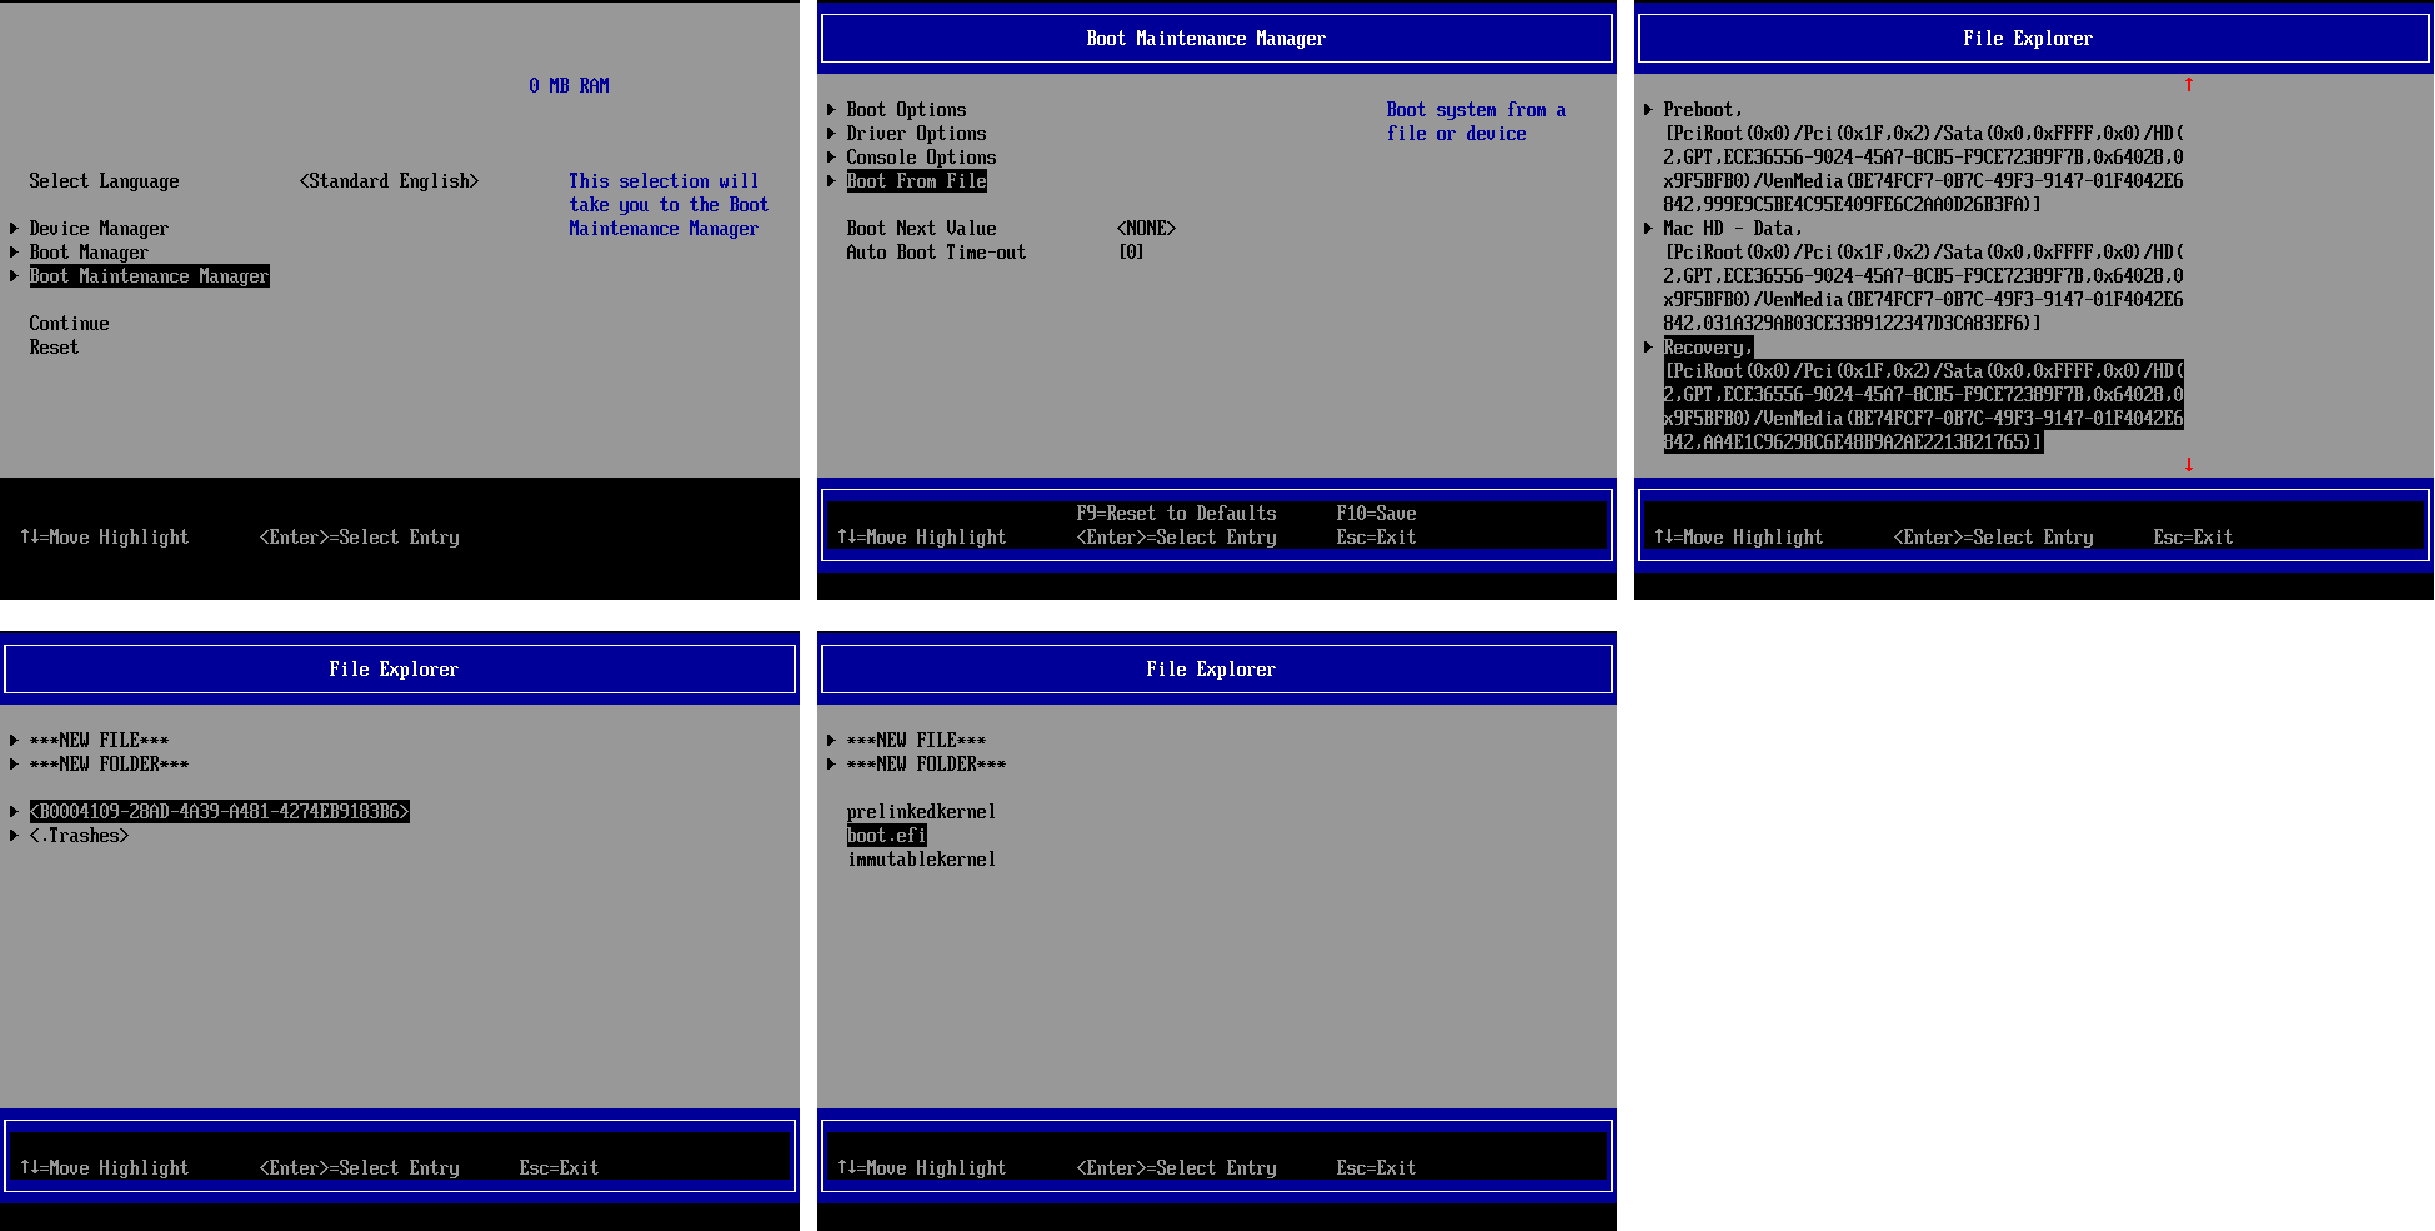
\includegraphics[width=\textwidth]{bios.pdf}
  \caption{进入Mac的Recovery模式。\textit{开启Mac虚拟机,使用“Windows+R”热键进入到虚拟机的BIOS系统,选择“Boot Maintenance Manager”进入。
  选择“Boot From File”选项,找到带有“Recovery.”的进入,选择其中的“boot.efi”文件启动,即可进入Recovery模式。}}\label{fig:bios}
\end{figure*}

%%%%%%%%%%%%%%%%%%%%%%%%%%%%%%%%%%%%%%%%%%%%%%%%%

\section{总结}\label{sec:Conclusion}

本文基于工作站虚拟机软件Virtual Box ,介绍了虚拟机的安装与使用,并根据实际操作的过程中遇到的问题进行了总结和整理。
总体来说,创建Ubuntu的虚拟机要易于创建macOS的虚拟机,同样的问题在不同的操作系统中的解决方案不尽相同。
通过本次实际操作,我对虚拟机的认识和理解得到了进一步的提高,同时也加深了对Linux、Mac OS X 等类Unix系统的认识。

\cleardoublepage \def\cleardoublepage{\clearpage\if@twoside \ifodd\c@page\else \hbox{}\newpage\if@twocolumn\hbox{}\newpage\fi\fi\fi}

{\small
\bibliographystyle{ieee}
\bibliography{main}
}

% @electronic{标识符,
%     url     =   {{网址}},
%     title   =   {{网站标题}}
% }
% @book{标识符,
%     title  = {{书籍标题}},
%     author = {{姓, 名 and ... and 姓, 名}},
%     publisher = {{出版社名称}},
%     year    =   {年份}
% }
% @inproceedings{标识符,
%     author      =   {{姓, 名 and 姓, 名 and ... and 姓, 名}},
%     title       =   {{论文标题}},
%     booktitle   =   {{会议论文集名称或会议名称}},
%     pages       =   {起始页码--终止页码},
%     year        =   {年份}
% }
% @article{标识符,
%     author  =   {{姓, 名 and 姓, 名 and ... and 姓, 名}},
%     title   =   {{论文标题}},
%     journal =   {{期刊名称}},
%     volume  =   {卷号},
%     number  =   {期号},
%     pages   =   {起始页码--终止页码},
%     year    =   {年份}
% }

% \end{CJK*}
\end{document}
